%\subsection{Objectives}
%
%The purpose of the experiment is to show the following points:
%\begin{itemize}
%\item the learning engine produces *accurate* and *concise* descriptions compared to a human
%expert's descriptions but costs just a fraction of the time; 
%\item it handles a variety of data formats; 
%\item the refinement step significantly improves the structure; 
%\item it is able to produce a description that is sufficiently accurate with 
%much smaller training sets (overfitting vs. underfitting); 
%\item demonstrate that there exists a correlation between sample size, execution time and accuracy,
%and the min sample size required to achieve certain accuracy correlates with the 
%data complexity.
%\end{itemize}

%% We conducted a series of experiments to study the learning algorithm
%% and measure its performance.
%%  In this section, we will show that
%% \begin{itemize}
%% \item the learning engine is capable of handing a variety of data formats;
%% \item while the initial structure discovery generates a reasonably
%% good candidate, the refinement phase significantly improves the
%% quality of the description through rewritings; 
%% \item the final output of the learning system is highly competitive
%% when compared with descriptions written by a human expert 
%% in terms of accuracy and conciseness; 
%% \item it is possible to learn from a small training set and produce
%% a relatively accurate description at a fraction of the cost;
%% \item there exists some correlation between the structural complexity
%% of the data and the minimum training size required to achieve certain
%% accuracy.
%% \end{itemize}

%% \subsection{Preliminaries}
\begin{table}
\begin{center}
\begin{tabular}{|l||c|l|} \hline
Data source		& KB/Chunks		& Description\\ \hline \hline
1967Transactions.short	& 70/999		& transaction records\\ \hline
MER\_T01\_01.cvs	& 22/491 	& comma-sep records\\ \hline
ai.3000			& 293/3000	& webserver log\\ \hline
asl.log 		& 279/1500	& log file of Mac ASL\\ \hline	
boot.log		& 16/262		& Mac OS boot log\\ \hline
crashreporter.log 	& 50/441 	& original crash log\\ \hline 
crashreporter.log.mod 	& 49/441	& modified crash log\\ \hline
sirius.1000		& 142/999 	& AT\&T phone\\
			&		& provision data\\ \hline
ls-l.txt		& 2/35		& Stdout from Unix\\
			&		& command ls -l\\ \hline
netstat-an		& 14/202		& output from netstat\\ \hline
page\_log		& 28/354		& printer logs\\ \hline
quarterlypersonalincome	& 10/62		& spread sheet\\ \hline 
railroad.txt		& 6/67		& US rail road info\\ \hline
scrollkeeper.log 	& 66/671		& application log\\ \hline
windowserver\_last.log 	& 52/680		& log from\\
                        &               & LoginWindow\\
                        &               & server on Mac\\ \hline
yum.txt			& 18/328		& log from pkg install\\ \hline
\end{tabular}
\caption{Benchmark profile including filename, size in KB, number of chunks
and brief description.} \shrink
\label{tab:benchmarks} 
\end{center}
\end{table}

%% 1967Transactions.short	& 70929		& transaction records \\ \hline
%% MER\_T01\_01.cvs	& 21731 	& comma-separated records\\ \hline
%% ai.3000			& 293460	& webserver log \\ \hline
%% asl.log 		& 279600	& log file of Mac ASL \\ \hline	
%% boot.log		& 16241		& Mac OS boot log \\ \hline
%% crashreporter.log 	& 50152 	& original crashreporter \\ 
%% 			&		& daemon log \\ \hline
%% crashreporter.mod 	& 49255		& modified crashreporter \\
%% 			&		& daemon log \\ \hline
%% sirius.1000		& 142607 	& AT\&T phone \\
%% 			&		& provision data \\ \hline
%% ls-l.txt		& 1979		& Stdout from Unix \\
%% 			&		& command ls -l \\ \hline
%% netstat-an		& 14355		& output from netstat \\ \hline
%% page\_log		& 28170		& printer logs \\ \hline
%% quarterlypersonalincome	& 10177		& spread sheet \\ \hline 
%% railroad.txt		& 6218		& US rail road info \\ \hline
%% scrollkeeper.log 	& 66288		& log from cataloging \\ \hline
%% windowserver\_last.log 	& 52394		& log from LoginWindow \\
%% 			&		& server on Mac \\ \hline
%% yum.txt			& 18221		& log from package installer\\ \hline
%	& \#  	 & Mode  &Header	& Array	& Group & Msgs 	
%	& 999	 & line	& no	& no	& no	& no	
%	& 491	 & line  & yes	& no	& yes	& no	
%	& 3000	 & line	& no	& no	& yes	& no	
%	& 1500	 & line	& no	& no	& yes	& no	
%	& 262	 & line	& no	& no	& no	& yes	
%	& 441	 & line	& no	& no	& no	& yes	
%	& 441	 & line	& no	& no	& no	& yes	
%	& 999	 & line	& yes	& yes	& no	& no	
%	& 35	 & line	& yes	& no	& no	& no	
%	& 202	 & block	& yes	& no	& no	& no	
%	& 354	 & line	& no	& no	& no	& no	
%	& 62	 & line	& yes	& no	& yes	& no	
%	& 67	 & line	& yes	& yes	& yes	& no	
%	& 671	 & line	& no	& no	& no	& yes	
%	& 680	 & line	& no	& no	& no	& yes	
%	& 328	 & line	& no	& no	& no	& no	

We conducted a series of experiments to study the correctness
and performance of our format inference algorithm.
Table~\ref{tab:benchmarks} lists the data sources we used in the experiments;
they range from system logs to application outputs to government
statistics. Except for sirius.1000, which is a proprietary format, the files 
are all available from \url{www.padsproj.org/learning.html}.
The size of the benchmarks varies from a few thousand lines to just a
few dozen.
%As we will see later,
%the size of the data source has implications in the training performance.
Most of the data files are ``line based,'' meaning that every line becomes a chunk
for the purposes of learning the format.  One exception is netstat-an, in which
chunks comprise multiple lines.
% Many of the formats include headers or footers which may complicate the descriptions.
% From a human point of view, sirius.1000 and railroad.txt consist of some special
% character separated arrays. Some data sources such as ai.3000 and asl.log
% contain groupings delimited by special characters such as [, ], or quotations.
% Many contain complex English text as logs or messages.
We include two versions of crashreporter.log: the original
``crashreporter.log'' and the slightly modified ``crashreporter.log.mod'' 
that we used as an example in this paper.  We include both to 
demonstrate that our minor modifications were simply for expository purposes.
%The latter has been used as an example in Section \ref{sec:review}. 

%\begin{table}
%\begin{center}
%\begin{tabular}{|l|c|c|c|} \hline
%		&  Time to prod.	& MDL score 	& Parsing accuracy 	\\ \hline
%HW IR	& -			& X		& -			\\ \hline	
%HW PADS	& X			& -		& X			\\ \hline	
%INF IR 	& -			& X		& -			\\ \hline
%INF PADS & X			& -		& X			\\ \hline 
%\end{tabular}
%\caption{Measurement for the representations} \label{tab:metrics}
%\end{center}
%\end{table}

%% For any of the given data sources, there exists four different representations in 
%% our experiments: hand-rewritten PADS by human expert (HW PADS), hand-rewritten IR directly
%% translated from the HW PADS (HW IR), inferred IR from the learning engine (Inf IR), and
%% inferred PADS description which is automatically translated from the Inf IR (Inf PADS). 
%% Note that as IR has a simplified language and is not as powerful as the full-fledged
%% PADS, the HW PADS does not use those features not available in IR and hence it is
%% not fully optimized. 
%% Nonetheless, the HW PADS and HW IR are thought to be ``pretty good'' descriptions of
%% the data and are used as control in the comparisons below. 
%% In general, we measure the time to produce the descriptions and parsing accuracy on
%% the HW PADS and Inf PADS and the MDL scores on the HW IRs and Inf IRs.
%% We measure accuracy by feeding the original data into the PADS accumulator tool.

% \subsection{Experiments}

\begin{table}
\begin{center}
\begin{tabular}{|l||c|c|c|c|} \hline
Data source			& SD(s)     & Ref(s) 	& Tot(s)  & HW(h)\\ \hline \hline
1967Transactions.short          & 0.20&      2.32&      2.56 	& 4.0 	 \\ \hline
MER\_T01\_01.csv                & 0.11&      2.80&      2.92 	& 0.5 	 \\ \hline
ai.3000                         & 1.97&      26.35&     28.64	& 1.0 	 \\ \hline
asl.log                         & 2.90&      52.07&     55.26	& 1.0 	 \\ \hline
boot.log                        & 0.11&      2.40&      2.53 	& 1.0 	 \\ \hline
crashreport.log                 & 0.12&      3.58&      3.73 	& 2.0 	 \\ \hline
crashreport.log.mod             & 0.15&      3.83&      4.00 	& 2.0 	 \\ \hline
sirius.1000                     & 2.24&      5.69&      8.00 	& 1.5 	 \\ \hline
ls-l.txt                        & 0.01&      0.10&      0.11 	& 1.0 	 \\ \hline
netstat-an                      & 0.07&      0.74&      0.82 	& 1.0 	 \\ \hline
page\_log                       & 0.08&      0.55&      0.65 	& 0.5 	 \\ \hline
quarterlypersonalincome         & 0.07&      5.11&      5.18 	& 48  	 \\ \hline
railroad.txt                    & 0.06&      2.69&      2.76 	& 2.0 	 \\ \hline
scrollkeeper.log                & 0.13&      3.24&      3.40 	& 1.0 	 \\ \hline
windowserver\_last.log          & 0.37&      9.65&      10.07	& 1.5 	 \\ \hline
yum.txt                         & 0.11&      1.91&      2.03 	& 5.0     \\ \hline
\end{tabular}
\vskip 0.25ex
\caption{Execution times. SD: time for structure-discovery phase; Ref: time for scoring and 
refinement; Tot: end-to-end time for complete inference algorithm; HW: 
time taken {\em in hours} to hand-write the corresponding description.} \shrink
\label{tab:times}
\end{center}
\end{table}

%% \begin{table}
%% \begin{center}
%% \begin{tabular}{|l||r|r|r|} \hline
%% Data source 			   & Inf 		&Ref 		& HW 	 \\ \hline \hline
%% 1967Transactions.short          & 0.295 		&0.218 		&0.268	 \\ \hline
%% MER\_T01\_01.csv                & 0.648 		&0.112		&0.138	 \\ \hline
%% ai.3000                         & 0.503		&0.332		&0.338	 \\ \hline
%% asl.log                         & 0.630		&0.267		&0.361	 \\ \hline
%% boot.log                        & 0.620		&0.481		&0.703	 \\ \hline
%% crashreport.log                 & 0.607		&0.328		&0.348	 \\ \hline
%% crashreport.log.mod             & 0.612		&0.329		&0.347	 \\ \hline
%% sirius.1000                     & 0.602		&0.470		&0.438	 \\ \hline
%% ls-l.txt                        & 0.559		&0.333		&0.401	 \\ \hline
%% netstat-an                      & 0.413		&0.394		&0.319	 \\ \hline
%% page\_log                       & 0.540		&0.107		&0.353	 \\ \hline
%% quarterlypersonalincome         & 0.544		&0.367		&0.354	 \\ \hline
%% railroad.txt                    & 0.715		&0.506		&0.522	 \\ \hline
%% scrollkeeper.log                & 0.625		&0.354		&0.352	 \\ \hline
%% windowserver\_last.log          & 0.618		&0.241		&0.267	 \\ \hline
%% yum.txt                         & 0.827		&0.305		&0.474	 \\ \hline
%% \end{tabular}
%% \caption{Normalized MDL Scores}
%% \label{tab:scores}
%% \end{center}
%% \end{table}

\paragraph*{Performance.}
Our first set of experiments measures the time required to infer a description
from example data.  In all our experiments, we used an 
Apple PowerBook G4 with a 1.67~GHz Processor and 512~MB DDR RAM 
running on Mac OSX 10.4 Tiger. Table \ref{tab:times} presents the execution times
for the structure-discovery phase (SD), the refinement phase (Ref) and the
total (Tot) end-to-end time of the algorithm including printing \pads{} descriptions and other 
overhead, all measured in seconds.  For accurate timing measurements, we ran the algorithm
10~times, and found the average after removing the best and the worst times.

There are two main lessons to take away from this initial set of
benchmarks.  First, the overall time to infer the structure of any our
example files was less than a minute, and was less than 10 seconds
except on a couple of the larger files.  Hence, although we have spent
very little time optimizing our algorithm, it already appears
perfectly capable of being used in real time by a programmer wishing
to understand and process small ad hoc data files.  Second, discovery
of an initial format is usually very fast, taking less than 3 seconds
in all cases.  Most of the algorithm's time is spent in format rewriting, which
often takes a factor of 10 or more time than structure discovery.  Moreover, most of the
rewriting time is taken in the data analysis phase (numbers not
shown).  Consequently, if format rewriting (particularly the data analysis phase)
is taking too long, the user may abort it to produce a 
slightly less refined description that may nevertheless be perfectly sufficient.

To give a very rough idea of how using the inference system compares with programming
descriptions by hand, we also measured the time it took for a person to write descriptions of
all of the data sources (See Table \ref{tab:times} again).  
Initially, our programmer (a Ph.D. in computer science)
knew very little about how the \pads{} system
worked in practice, having only read a few of our conference papers.  Consequently, writing
the first description took a long time, approximately 48 hours (two days of working at
an ``ordinary'' pace) for quarterlypersonalincome.  While different people with different 
backgrounds will clearly learn at different rates, there is little doubt that the
format inference algorithm is a tremendous benefit to novices, particularly
to those data analysts without a Ph.D. in computer science, who are uninterested
in learning some new data description language.  After some practice, our programmer was
able to write most descriptions in 1 to 2 hours, so generating descriptions in a few
seconds still has great benefit, even to experts.

\begin{figure}
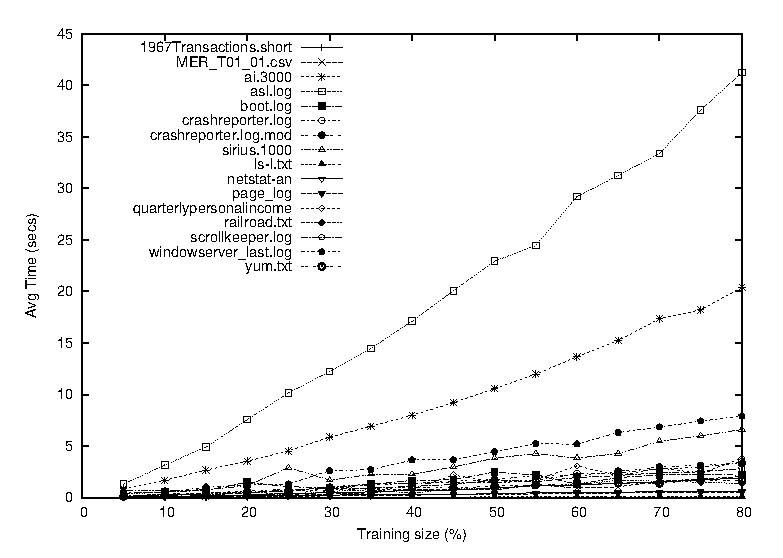
\epsfig{file=traintime.eps, width=\columnwidth}
\caption{Execution times of training sets} \label{fig:traintime} \shrink
\end{figure}

To understand the scaling behavior of our algorithm, we
randomly selected 5\%, 10\%, 15\%, ..., 80\% of the chunks in every data source
and measured the performance of the algorithm on each subset of the data that was
selected. Figure \ref{fig:traintime}
plots the execution time against the percentage of each data source selected.
These experiments suggest that once a format is fixed, the cost of inference
grows linearly with the amount of data.  However, it is also clear that the raw
size of the data is not the only factor determining performance.  The nature and complexity
of the format is also a significant factor.  For instance, windowserver\_last.log
is only one third the size of sirius.1000, but takes substantially longer 
for the inference algorithm to process.

\paragraph*{Correctness.}
To evaluate the correctness of our algorithm, we again selected
random subsets of each data source, trained our algorithm on those subsets and
measured the error rate of the inferred parser on the remaining data.
Figure \ref{fig:trainsucc} graphs the percentage of successfully parsed records
versus the percentage of the data used in training.  Note
that accuracy does not uniformly improve.  This variation is caused by the
randomness in our data selection and the fact that in some cases,
we have very small absolute quantities of data relative to the
underlying complexity of the formats.   
For instance, at 5\% training size, ls-l.txt is just one line of data.
%In practice, there is no reason why a programmer would attempt to learn
%a format from such a small amount of data -- he or she might as well train on the entire
%ls-l.txt file (it only takes a 10th of a second to do so). Nevertheless, we
%present the results of all experiments uniformly.

To understand the correctness properties of our algorithm from a different angle,
we record the minimum training sizes in percentages required to achieve 90\% and 95\% accuracy for
all the benchmarks in Table \ref{tab:correlate}.  This table also reports the
normalized cost of a description (\normcostdescription), which we compute by dividing the
first component of the information-theoretic score in \secref{sec:score} 
by the number of bits in the data.  \normcostdescription~ gives
a rough indication of the complexity of the data source. The higher the
normalized score, the more complicated the data, and the greater the fraction of data is
needed to learn an accurate description.  The rows of of Table \ref{tab:correlate}
are sorted in ascending NS score.  From the table, one can see that ls-l.txt and
railroad.txt have high NS scores.  This is because they are quite small data sources
(2KB and 6KB respectively), yet have relatively complicated formats.  Consequently,
it takes a substantial portion of the data to learn an accurate parser.  For most of the other
data sources, a substantially smaller percentage of the data is required to achieve
high accuracy.  Overall, for 11 of 16 benchmarks, less than
15\% of the data is needed to achieve 95\% accuracy or more.

\begin{figure}
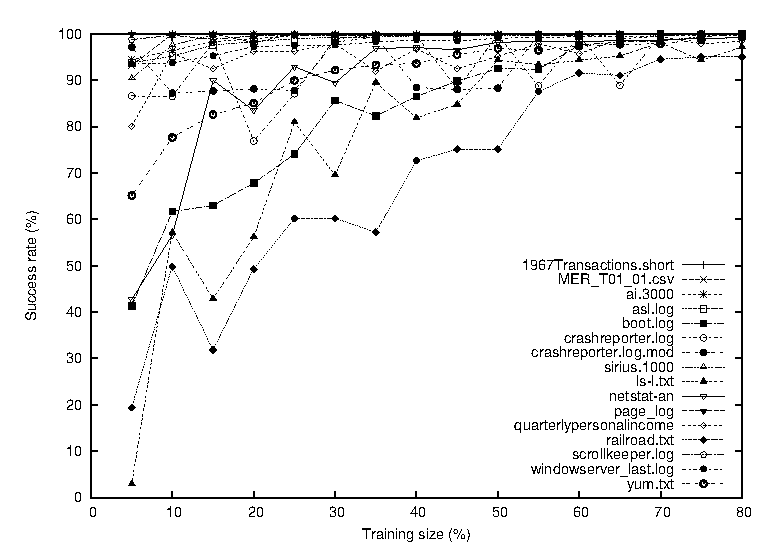
\epsfig{file=successrate.eps, width=\columnwidth}
\caption{Success rates of training sets} \label{fig:trainsucc} \shrink
\end{figure}

\begin{table}
\begin{center}
\begin{tabular}{|l||c|c|c|} \hline
Data source	        & \normcostdescription  	& 90\% 		& 95\% \\ \hline \hline
sirius.1000             & 0.0001  	& 5		& 10 \\ \hline
1967Transactions.short	& 0.0003  	& 5		& 5 \\ \hline
ai.3000                 & 0.0004  	& 5		& 10 \\ \hline
asl.log                 & 0.0012  	& 5		& 10\\ \hline
scrollkeeper.log        & 0.0020  	& 5		& 5\\ \hline
page\_log               & 0.0032  	& 5		& 5\\ \hline
MER\_T01\_01.csv        & 0.0037  	& 5		& 5 \\ \hline
crashreporter.log       & 0.0052  	& 10		& 15\\ \hline
crashreporter.log.mod   & 0.0053  	& 5		& 15\\ \hline
windowserver\_last.log  & 0.0084  	& 5		& 15\\ \hline
netstat-an              & 0.0118  	& 25		& 35\\ \hline
yum.txt                 & 0.0124  	& 30		& 45\\ \hline
quarterlypersonalincome & 0.0170  	& 10		& 10\\ \hline
boot.log                & 0.0213  	& 45		& 60\\ \hline
ls-l.txt                & 0.0461  	& 50		& 65 \\ \hline
railroad.txt            & 0.0485  	& 60		& 75\\ \hline
\end{tabular}
\caption{Correctness measures.  \normcostdescription: normalized cost of description;
Min Training size (\%) to obtain required accuracy} \shrink
\label{tab:correlate}
\end{center}
\end{table}


%% We also show the type complexity 
%% (measuring the complexity the description) and the normalized structural variance (measuring
%% how many disjoint paths the original data records take in the structure normalized by number of
%% chunks) side-by-side with the
%% minimum training sizes. We sort the rows by increasing type complexity and see a rough
%% positive correlation between the structural complexity and the minimum training size required,
%% with the exception of quarterlypersonalincome.
%% Quarterlypersonalincome is special as it has only 62 records, 
%% but each record is represented by a very big structure, therefore the normalized
%% type complexity is large even though the data are quite uniform and easy to learn.

%% To find out what the system can learn from smaller sample data,
%% we select random training sets of 5\%, 10\%, 15\%, ..., 80\% of 
%% the original data (three sets for each size) and run learning tool end to end on 
%% them and take the average values of the three sets for each training size. 
%% Figure \ref{fig:trainsucc} and Figure \ref{fig:traintime} plot the average 
%% parsing accuracy and execution time against the various training set sizes.
%% The intuition that learning accuracy is proportional to the training sizes is
%% confirmed here though the relationship is not necessarily linear. Some of the
%% data such as ls-l.txt, boot.log and railroad.txt are more difficult to train
%% than others. In these cases, the training sets are too small 
%% given the complexity and the large variance of data (see Table \ref{tab:correlate}).
%% For instance, at 5\% training size, ls-l.txt has just one line of record. 
%% Not surprisingly, our system couldn't get anything but this line right, and
%% hence produces poor result. There are some dips in the curves in Figure \ref{fig:trainsucc}.
%% They exist because some random samples does not provide good coverage of the data.
%% These are not anomalies because the lower accuracy is still way higher than the 
%% training size. 

%% The training time is evidently linear to the training size from the plot. Larger
%% and more complex data like asl.log and ai.3000 takes more time to learn, which
%% is intuitively correct.

%% Data source		  & NS  	& Var		& 90\% 		& 95\% \\ \hline \hline
%% sirius.1000            & 0.0001	& 0.0050	& 5		& 10 \\ \hline
%% 1967Transactions.short	& 0.0003	& 0.0020	& 5		& 5 \\ \hline
%% ai.3000                 & 0.0004	& 0.0037	& 5		& 10 \\ \hline
%% asl.log                 & 0.0012	& 0.0133	& 5		& 10\\ \hline
%% scrollkeeper.log        & 0.0020	& 0.0089	& 5		& 5\\ \hline
%% page\_log               & 0.0032	& 0.0085	& 5		& 5\\ \hline
%% MER\_T01\_01.csv        & 0.0037	& 0.0122	& 5		& 5 \\ \hline
%% crashreporter.log       & 0.0052	& 0.0181	& 10		& 15\\ \hline
%% crashreporter.log.mod   & 0.0053	& 0.0181	& 5		& 15\\ \hline
%% windowserver\_last.log  & 0.0084	& 0.0279	& 5		& 15\\ \hline
%% netstat-an              & 0.0118	& 0.0693	& 25		& 35\\ \hline
%% yum.txt                 & 0.0124	& 0.0732	& 30		& 45\\ \hline
%% quarterlypersonalincome & 0.0170	& 0.0806	& 10		& 10\\ \hline
%% boot.log                & 0.0213	& 0.0725	& 45		& 60\\ \hline
%% ls-l.txt                & 0.0461	& 0.2571	& 50		& 65 \\ \hline
%% railroad.txt            & 0.0485	& 0.1940	& 60		& 75\\ \hline


%% Finally, we record the minimum training sizes required to achieve 90\% and 95\% accuracy for
%% all the benmarks in Table \ref{tab:correlate}. We also show the normalized type complexity 
%% (measuring the complexity the description) and the normalized structural variance (measuring
%% how many disjoint paths the original data records take in the structure normalized by number of
%% chunks) side-by-side with the
%% minimum training sizes. We sort the rows by increasing type complexity and see a rough
%% positive correlation between the structural complexity and the minimum training size required,
%% with the exception of quarterlypersonalincome.
%% Quarterlypersonalincome is special as it has only 62 records, 
%% but each record is represented by a very big structure, therefore the normalized
%% type complexity is large even though the data are quite uniform and easy to learn.

%\begin{figure}
%\begin{center}
%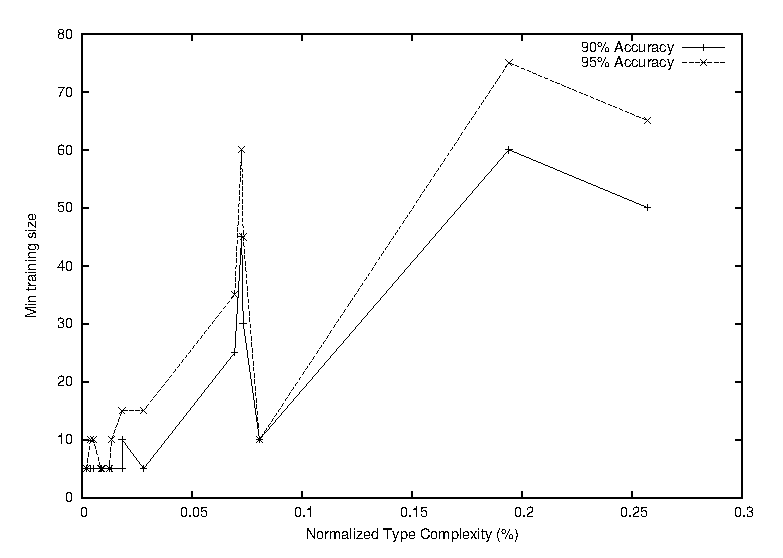
\epsfig{file=traintycomp.eps, width=\columnwidth}
%\caption{Correlation between structure complexity of 
%the data and minimum training size required}
%\end{center}
%\end{figure}


%% We first hand-coded all 16 formats in PADS and IR and measure timings and the scores 
%% of supposedly good descriptions (see HW column in Table \ref{tab:times}). 
%% Several formats takes a few hours and up to 2 days(!) to complete because these were the very first 
%% PADS descriptions ever written by this person. It is obvious that coding description
%% in PADS is a daunting task for a novice despite that he is a computer science PhD!
%% To score a given HW IR, we wrote a simple recursive-descent parser with backtracking
%% for our IR so that the original data can be populated into the IR structure for
%% correct scoring of the data complexity which is the second component of the MDL score.
%% After a few attempts and modifications, the HW PADS descriptions parses all 
%% the original data files with 100\% accuracy.

%% Next we ran the learning system on all 16 data files in their entirety, 
%% measured timings for structure inference, refinement and the total time which includes
%% printing out the PADS descriptions and other overhead. 
%% We also recorded the scores of both the initial structure and the final structure after refinement.
%% All these measurements are included in Table \ref{tab:scores}.
%% The generated PADS descriptions parses all original data files with 100\% accuracy,
%% therefore the correctness of the learned formats is guaranteed.

%% We can see from Table \ref{tab:scores} that the learning system
%% generates correct descriptions of any given data in matters of seconds as opposed to
%% the hours and days taken by human beings. The execution time is roughly proportional
%% to the size of input data. For example, the largest data sources, ai.3000 and asl.log,
%% take also the longest time. Refinement typically takes more time than initial
%% structure discovery, as the functional dependency analysis in this phase is a quadratic
%% in the number of nodes in the IR and is the bottleneck of the algorithm. 
%% Note that all these timings are achieved with a completely unoptimized prototype system
%% with lots of overhead in book-keeping and I/Os.

%% It is interesting to see that the learning system generally produces descriptions
%% with a better score than the handwritten ones, sometimes even by a large margin, such
%% as in boot.log and page\_log. This is often due to the following reasons.

%% \begin{itemize}
%% \item The HW IR were not optimized by the MDL scores but instead
%% by the expert's intuition, therefore often more type complexity optimized than
%% data complexity optimized but data complexity usually outweigh the type
%% complexity in the overall scores.
%% However, for most of the data sources, the final scores for HW IR and Inf IR were so close 
%% that we are confident that the scoring function we use here is meaningful.

%% \item Human expert pay more attention to the semantics of the formats and 
%% tries to generalize the structure. For example, in sirius.1000, the
%% HW IR has a zip field, while in the data itself, the zip field is always
%% blank. The inferred IR fixed the zip field to be
%% blank because it doesn't have the data to infer otherwise. 
%% In another example, the HW IR of boot.log describes the log message part 
%% as a \verb#StringME /.*/# because the human expert knows anything
%% message could have occurred in that position, so \verb#/.*/# is the safest thing
%% to do, despite it being more data complex. 
%% The inferred description, on the other hand, tend to overfit data,
%% and may refine types that should not be refined. Similar things happen
%% in the HW IR for page\_log where {\tt Pstring} is used instead of constant strings, 
%% which results in higher scores.

%% \item Due to the restriction of the IR language, certain tweaks, including the
%% use of regular expressions in the HW IRs are necessary to enable
%% the data population. Such tweaks are often not optimized and introduce
%% additional complexity to the HW IR. 
%% \end{itemize}

%Compare these with the golden numbers from (1) in a big table. Show that the difference in scores
%can be significant in some cases hence room for improvement (may go into the discussion section)
%but timing advantage is huge and refinement improves initial struct a lot. Maybe also compare a case or
%two where the score from silver is comparable to golden and the actually description produced is also
%close to golden (to demo that our scoring makes some sense).
%Have a discussion here about while the learning tool may produce a longer description than human does,
%it parses all data correctly so the user is getting all these for free which is a tremendous benefit.
%Discuss 1967 where the inference does better than human.
